\title{\textsc{Corn}}
\author{Giorgio Giuffr\`e}
\date{}

\documentclass{article}
\usepackage[utf8]{inputenc}
\usepackage{mathtools}
\usepackage{amssymb}
\usepackage{tikz}
\usepackage{tkz-graph}
\usepackage{hyperref}

\renewcommand*{\EdgeLineWidth}{0.16pt}
\renewcommand{\labelitemi}{$\cdot$}

\tikzset{
	every neuron/.style={
		circle,
		draw,
		minimum size=1cm
	},
	neuron missing/.style={
		draw=none, 
		scale=4,
		text height=0.333cm,
		execute at begin node=\color{black}$\vdots$
	},
}



\begin{document}
\maketitle



%%% ========================================
%%% ========================================

\begin{abstract}
\textsc{Corn} (COstruttore di Reti Neurali) è una piccola piattaforma che permette di progettare e allenare semplici reti neurali artificiali feedforward (cioè acicliche), e di collaudarle poi su input numerici.
\end{abstract}



%%% ========================================
%%% ========================================

\section{Introduzione}

\subsection{Cos'è una rete neurale?}

\paragraph{} Il miglior esempio di rete neurale è senza dubbio il cervello umano: una rete di cellule collegate tra loro --- dette \emph{neuroni} --- che si scambiano informazione sotto forma di segnali elettrici. Alcuni neuroni si interfacciano con l'ambiente esterno: sono i neuroni sensoriali (di input) e quelli motori (di output); altri invece stanno “nascosti” all'interno, nei meandri della rete. Possiamo vedere i neuroni di input e quelli di ouput come l'\textit{interfaccia} della rete con l'utente, mentre i neuroni nascosti costituiscono l'\textit{implementazione} di un algoritmo --- il comportamento umano, nel caso del nostro cervello. Nel cervello, ogni neurone manda un segnale a più neuroni e riceve segnali da neuroni diversi, determinando un'intricata catena parallela di segnali che termina con i neuroni motori, collegati ai muscoli.

\paragraph{} Formalmente, una rete neurale è un grafo orientato in cui ogni nodo è un \textbf{neurone} e ogni arco è un \textbf{collegamento} che va da un neurone a un altro. Un neurone è una cellula che riceve uno o più segnali di input, li somma ed emette un solo segnale di output (quindi un neurone è una funzione $f : \mathbb{R}^n \rightarrow \mathbb{R}$, dove $n \ge 1$ è il numero di segnali in ingresso). In base al segnale totale di input $x$, ogni neurone emette quindi un certo segnale di output $f(x)$ che può poi ramificarsi, cioè può essere mandato a più di un neurone, a seconda di com'è disegnato il grafo. Le connessioni (gli archi) tra un neurone e l'altro sono pesate, cioè ogni input $x_i$ viene moltiplicato per una costante reale $w_i$ che può essere modificata dalla rete nel corso del tempo.

\paragraph{} Tutti i neuroni della rete implementano la stessa semplice funzione $f$, detta \textbf{funzione di attivazione}. Chiaramente, l'output di due neuroni può essere diverso, per il fatto che gli archi della rete non hanno tutti lo stesso peso. La capacità della rete di modificare i pesi delle proprie connessioni fa sì che essa sia capace di associare ad ogni input un certo output desiderato. Ad esempio, una rete con due neuroni di input e un neurone di output può modificare i propri pesi in modo da imparare a calcolare la media di due numeri che le vengono dati in input:

\begin{center}
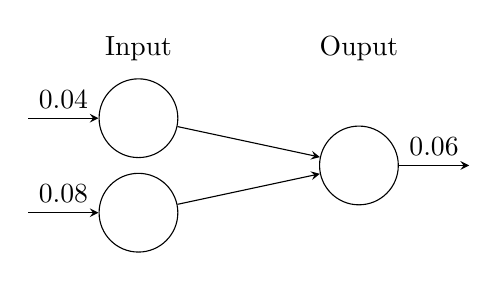
\begin{tikzpicture}[x=1.4cm, y=1.2cm, >=stealth]

\foreach \m/\l [count=\y] in {1,2}
	\node [every neuron/.try, neuron \m/.try] (input-\m) at (0,2-\y) {};

\foreach \m [count=\y] in {1}
	\node [every neuron/.try, neuron \m/.try ] (output-\m) at (2,1.5-\y) {};

\foreach \l [count=\i] in {0.04, 0.08}
	\draw [<-] (input-\i) -- ++(-1,0)
		node [above, midway] {$\l$};

\foreach \l [count=\i] in {0.06}
	\draw [->] (output-\i) -- ++(1,0)
		node [above, midway] {$\l$};

\foreach \i in {1,2}
	\foreach \j in {1}
		\draw [->] (input-\i) -- (output-\j);

\foreach \l [count=\x from 0] in {Input, Ouput}
	\node [align=center, above] at (\x*2,1.5) {\l};

\end{tikzpicture}
\end{center}

La rete apprende grazie ad una serie di \textbf{esempi} che le vengono presentati: $(0.04, 0.08 \rightarrow 0.06)$, $(0.05, 0.01 \rightarrow 0.03)$, $(0.02, 0.05 \rightarrow 0.035)$, $(0.09, 0.08 \rightarrow 0.085)$ e così via. Più esempi vengono forniti, più è preciso l'apprendimento. A questo proposito, è importante notare che la rete fornisce risposte \textit{approssimate}, dovendo imparare da un insieme di esempi anziché da delle regole esplicite.

\paragraph{} Oppure, una rete con 4 neuroni in ingresso e 4 in uscita (più un livello di neuroni “nascosti”) potrebbe imparare a calcolare il successore di un numero in formato binario\footnote{I pallini neri nel disegno indicano la presenza di eventuali altri neuroni nascosti, oltre ai due disegnati}:

\begin{center}
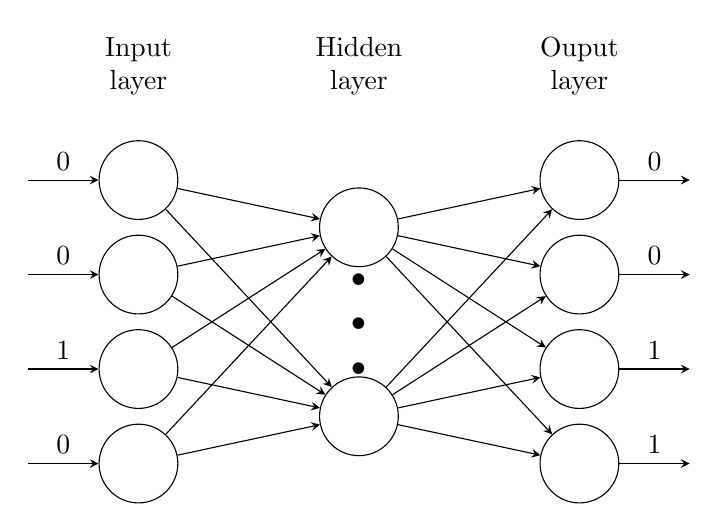
\begin{tikzpicture}[x=1.4cm, y=1.2cm, >=stealth]

\foreach \m/\l [count=\y] in {1,2,3,4}
	\node [every neuron/.try, neuron \m/.try] (input-\m) at (0,2-\y) {};

\foreach \m/\l [count=\y] in {1,missing,2}
	\node [every neuron/.try, neuron \m/.try] (hidden-\m) at (2,1.5-\y) {};

\foreach \m [count=\y] in {1,2,3,4}
	\node [every neuron/.try, neuron \m/.try ] (output-\m) at (4,2-\y) {};

\foreach \l [count=\i] in {0,0,1,0}
	\draw [<-] (input-\i) -- ++(-1,0)
		node [above, midway] {$\l$};

\foreach \l [count=\i] in {0,0,1,1}
	\draw [->] (output-\i) -- ++(1,0)
		node [above, midway] {$\l$};

\foreach \i in {1,...,4}
	\foreach \j in {1,...,2}
		\draw [->] (input-\i) -- (hidden-\j);

\foreach \i in {1,...,2}
	\foreach \j in {1,...,4}
		\draw [->] (hidden-\i) -- (output-\j);

\foreach \l [count=\x from 0] in {Input, Hidden, Ouput}
	\node [align=center, above] at (\x*2,1.8) {\l \\ layer};

\end{tikzpicture}
\end{center}

\subsection{Cosa può fare \textsc{Corn}?}

\paragraph{} Insomma, i compiti che una rete può imparare sono numerosissimi e \textsc{Corn} offre un'interfaccia semplice per specificare sia la configurazione della rete sia i compiti da farle imparare. La progettazione di una rete neurale artificiale si articola in tre fasi: Definizione dell'architettura della rete; definizione degli esempi da presentare alla rete; allenamento della rete. Una volta allenata la rete, la si può interrogare su degli input numerici.



%%% ========================================
%%% ========================================

\section{Guida per l'utente}

\paragraph{} \textsc{Corn} consiste di una sola finestra principale, dalla quale l'utente può lavorare su una rete alla volta. La finestra principale presenta, a sinistra, un elenco di cartelle contenenti le reti finora create (oltre a quelle disponibili di default). Ci sono tre cartelle, corrispondenti ai tre tipi di rete che il programma gestisce: le reti con funzione di attivazione sigmoide, quelle ad arcotangente e quelle a tangente iperbolica. Basta cliccare su una cartella e poi su una rete dell'elenco per potersi interfacciare con essa.

\paragraph{} Come detto prima, la progettazione di una rete si articola in tre semplici fasi:
\begin{itemize}
	\item definizione dell'architettura della rete;
	\item definizione degli esempi su cui la rete si allenerà;
	\item allenamento vero e proprio.
\end{itemize}
La prima cosa da fare, quindi, è andare sul menù “Rete” e cliccare “Nuova Rete”. La finestra principale contiene ora un pannello dal quale possiamo costruire la rete. Innanzitutto bisogna decidere il \textbf{nome} con cui battezzare la rete (senza l'estensione \textit{.net}, aggiunta automaticamente per memorizzarla in un file); è utile darle il nome del compito che deve imparare: ad esempio, una rete che debba apprendere a calcolare la somma tra quattro numeri potrebbe chiamarsi “sum\_4”, per poterla ritrovare poi con più facilità. Si deve poi selezionare il \textbf{tipo di funzione di attivazione} dei neuroni (la stessa funzione per tutti i neuroni: ciò che cambia sono solo i pesi delle connessioni) e infine il \textbf{numero di livelli} della rete (includendo nel conto il livello di input e quello di output). Più il compito è elaborato, più livelli ci vogliono; generalmente, uno o due livelli nascosti vanno più che bene ma, se l'utente vuole sperimentare, può selezionare fino a 8 livelli. Cliccando “Prosegui...”, l'utente potrà poi specificare il \textbf{numero di neuroni} per ogni livello; i livelli sono ordinati dall'input all'output e i più importanti sono il primo e l'ultimo, che dovranno contenere rispettivamente il numero di neuroni in ingresso e il numero di neuroni in uscita. Ora, basta cliccare “Crea” e la nuova rete comparirà in una cartella dell'elenco delle reti, a sinistra nella finestra principale.

\paragraph{} Per scrivere gli esempi da presentare alla rete, dal menù “Dati” si seleziona “Nuovo foglio di esempi”. Quello che viene presentato all'utente è un editor di testo diviso in due parti: nella prima va inserito l'input del singolo esempio; nella seconda l'output desiderato. Input e output devono essere sequenze di uno o più numeri floating point e bisogna tenere presente che i valori ideali per questi numeri sono tra 0 e 1 (per le reti a sigmoide, che hanno codominio $[0,1]$) oppure tra -1 e 1 (per le reti ad arcotangente o a tangente iperbolica, con codominio $[-1,1]$); va quindi benissimo anche una codifica binaria (solo 0 e 1) o bipolare (solo -1 e 1), per apprendere funzioni booleane o quant'altro. Ogni esempio va aggiunto con “Aggiungi” e dopo aver aggiunto l'ultimo basta cliccare “Crea” e rispondere alla finestra di dialogo indicando il nome del foglio di esempi (aggiungendo anche l'estensione \textit{.data}). Ancora, è opportuno dare il nome del compito da imparare: un foglio di esempi per la media tra due numeri si potrebbe intitolare “avg\_2” o “media”.

\paragraph{} Dobbiamo ora allenare la nostra rete --- i cui pesi sono ora casuali --- con il foglio di esempi appena creato. Per fare ciò navighiamo nell'elenco di reti a sinistra fino a trovare la rete che cerchiamo. Si apre ora l'interfaccia utente-rete, dalla quale possiamo scegliere se allenare la rete o interrogarla su degli input: basta scegliere tra le due tab in alto. Può essere interessante collaudare la rete prima ancora di averla allenata: darà degli output insensati per via del fatto che i pesi delle sue connessioni sono stati inizializzati a caso. Per allenarla, invece, inseriamo il nome del \textbf{file di dati} da cui la rete imparerà, il \textbf{massimo numero di epoche}\footnote{Un'epoca è il periodo in cui la rete osserva tutti gli esempi di un foglio: dopo tre epoche, la rete avrà visto ogni esempio tre volte.} che la rete avrà a disposizione per allenarsi e il massimo \textbf{errore} (medio, calcolato sugli esempi) tollerato. Schiacciando il pulsante “Allena”, la rete apprenderà il compito richiesto grazie all'algoritmo di \emph{Backpropagation}\footnote{\url{https://en.wikipedia.org/wiki/Backpropagation}}. L'algoritmo può impiegare pochi millisecondi come anche parecchi secondi: ciò dipende dalla difficoltà del compito che la rete deve imparare e, soprattutto, dall'architettura della rete: più neuroni ci sono, più l'algoritmo è lento.

\paragraph{} Per testare la rete che abbiamo appena allenato, selezioniamo l'altra tab (“Collauda la Rete”) dell'interfaccia utente-rete. Qui l'utente può mettere in input dei numeri (interi o reali, ma la rete li interpreta come reali) e premere “Vai” per osservare il risultato della rete. Si potrà notare come una rete allenata fornisca, con un certo grado di approssimazione, proprio gli output che è stata allenata a calcolare.

\paragraph{} Possiamo anche collegare diverse reti tra loro creando una \emph{inter-rete}. È sufficiente fare \emph{ctrl-click} (\emph{cmd-click} sul Mac) per aggiungere una rete dall'elenco a sinistra nell'inter-rete che stiamo creando. Dopo aver aggiunto le reti che ci servono, dobbiamo cliccare “Inter-rete” dal menù “Rete”. Ci viene presentata una tabella (la matrice di adiacenza dell'inter-rete): per collegare l'output della rete $x$ a un input della rete $y$ dovremo cliccare la casella $x$ della riga $y$, che si colorerà di nero. Un successivo click annulla il collegamento tra le due reti. Il pulsante “Collauda” porterà all'interfaccia per interrogare la rete appena creata, in cui si dovrà inserire un input di lunghezza pari alla somma dei neuroni di input delle reti in ingresso.



%%% ========================================
%%% ========================================

\section{Implementazione}

\paragraph{} Il programma è stato progettato seguendo lo schema \textit{Model-View} ed è diviso in due blocchi ben distinti: il modulo logico (nella cartella “logica”) e quello grafico. Il modulo logico è indipendente da quello grafico. Mentre l'interfaccia è in italiano, l'implementazione è in inglese. Sono stati usati \texttt{gcc 4.6} (con supporto parziale per \texttt{C++11}), \texttt{Qt 5.3.2} e \texttt{GNU Make 3.81} su Ubuntu 12.04.

\subsection{Parte logica}

\paragraph{} Una rete neurale è una rete, che a sua volta è un grafo orientato. Un grafo orientato è rappresentabile per mezzo della sua matrice di adiacenza $W$, in cui l'elemento $w_{ij}$ rappresenta la presenza o meno di un collegamento dal nodo $j$-esimo al nodo $i$-esimo. Per modellare una rete neurale, in cui i collegamenti tra i neuroni sono pesati, la matrice di adiacenza deve avere elementi reali (\texttt{float}): ogni segnale dal neurone $j$ al neurone $i$ verrà moltiplicato per $w_{ij}$.

\paragraph{} Alla base della gerarchia che implementa una rete neurale (in figura) sta la classe \texttt{DGraph} (\emph{Directed Graph}), sottotipo di \texttt{std::vector<std::vector<float> >}; è quindi una matrice di \texttt{float}. Non si sono scelti i \texttt{double} perché, anche biologicamente, una rete neurale non lavora a precisione elevata. \texttt{DGraph} implementa un grafo orientato ma \emph{non} aciclico, dato che in futuro il programma potrebbe essere dotato di reti cicliche (un'architettura ben più potente ma anche più complicata); per ora, la classe \texttt{layeredNetwork} implementa un'architettura che garantisce assenza di cicli. texttt{DGraph}, per ereditarietà, è un contenitore. Sono stati introdotti due nuovi iteratori per il seguente motivo: di ogni nodo interessano solo i collegamenti con gli \emph{altri} nodi; per questo, la classe \texttt{weights\_iterator} itera sui collegamenti entranti (anche nulli) di un particolare nodo (specificato nel costruttore dell'iteratore) ma evita automaticamente i collegamenti del nodo con se stesso. Per completezza, questa classe è definita a partire da \texttt{nodes\_iterator}, una semplice classe iteratore che rappresenta un indice da utilizzare con l'operatore di subscripting \texttt{[ ]} per iterare sui nodi.

\begin{center}
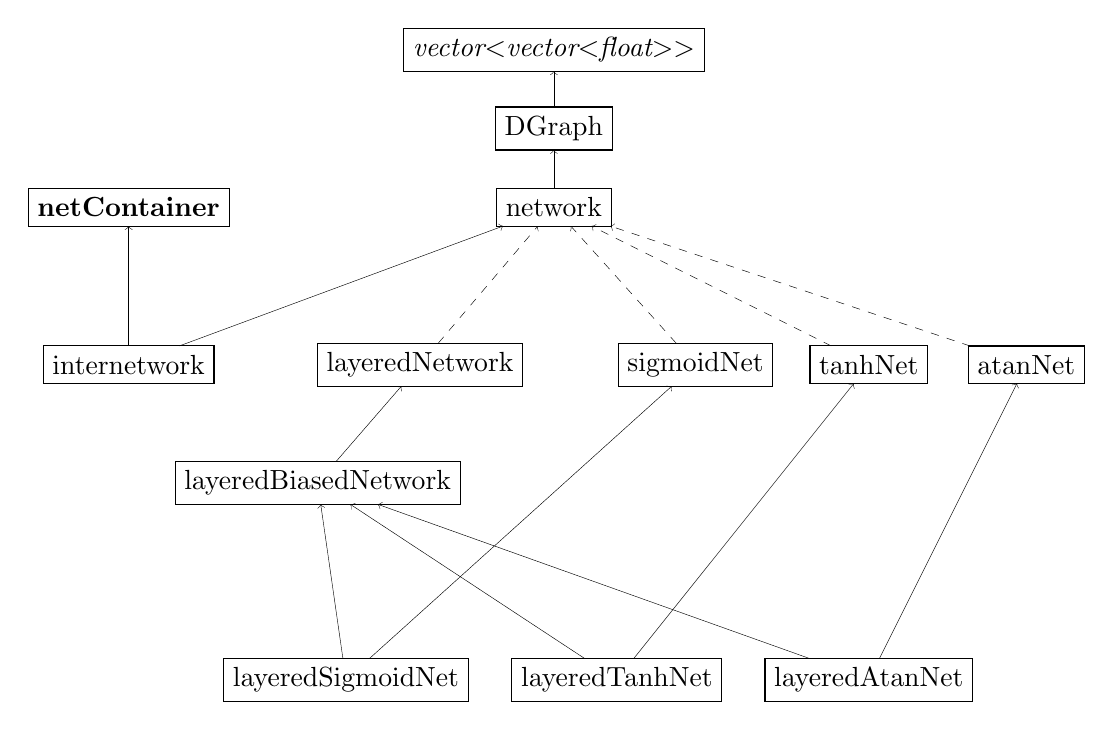
\begin{tikzpicture}
\tikzset{VertexStyle/.style = {shape=rectangle, fill=white, draw}}
\tikzset{EdgeStyle/.style = {->}}

\Vertex[L=\emph{vector$<$vector$<$float$>$$>$}]{vector}
	\Vertex[x=0,y=-1]{DGraph}
		\Vertex[x=0,y=-2]{network}
			\Vertex[x=-1.7,y=-4]{layeredNetwork}
				\Vertex[x=-3,y=-5.5]{layeredBiasedNetwork}
			\Vertex[x=1.8,y=-4]{sigmoidNet}
			\Vertex[x=4,y=-4]{tanhNet}
			\Vertex[x=6,y=-4]{atanNet}

					\Vertex[x=-2.64,y=-8]{layeredSigmoidNet}
					\Vertex[x=0.8,y=-8]{layeredTanhNet}
					\Vertex[x=4,y=-8]{layeredAtanNet}

		\Vertex[x=-5.4,y=-2,L=\textbf{netContainer}]{netContainer}
			\Vertex[x=-5.4,y=-4]{internetwork}

\Edge(DGraph)(vector)
\Edge(network)(DGraph)
\Edge[style={dashed}](layeredNetwork)(network)
\Edge(layeredBiasedNetwork)(layeredNetwork)
\Edge[style={dashed}](sigmoidNet)(network)
\Edge[style={dashed}](tanhNet)(network)
\Edge[style={dashed}](atanNet)(network)
\Edge(layeredSigmoidNet)(sigmoidNet)
\Edge(layeredSigmoidNet)(layeredBiasedNetwork)
\Edge(layeredTanhNet)(tanhNet)
\Edge(layeredTanhNet)(layeredBiasedNetwork)
\Edge(layeredAtanNet)(atanNet)
\Edge(layeredAtanNet)(layeredBiasedNetwork)
\Edge(internetwork)(network)
\Edge(internetwork)(netContainer)
\end{tikzpicture}
%\emph{\caption{Gerarchia del modulo logico (frecce tratteggiate indicano ereditarietà virtuale)} \label{fig:M1}}
\end{center}

\paragraph{} Da \texttt{DGraph} eredita la classe \texttt{network}, che implementa alcune funzionalità specifiche delle reti come il passaggio d'informazione (con \texttt{activation\_function}), l'inizializzazione dei pesi e il calcolo del flusso (\texttt{operator()}). Da \texttt{network} discendono varie classi:
\begin{itemize}
	\item \texttt{internetwork}: una \emph{rete di reti} --- un contenitore che è esso stesso rete;
	\item \texttt{layeredNetwork}, che definisce l'\textbf{architettura} a strati tipica delle reti neurali che creeremo;
	\item \texttt{sigmoidNet}, \texttt{tanhNet} e \texttt{atanNet}, che definiscono le \textbf{funzioni di attivazione} dei neuroni della rete.
\end{itemize}
È necessaria una classe ulteriore: \texttt{layeredBiasedNetwork}, che aggiunge un dettaglio tecnico alla classe da cui eredita, cioè la presenza di neuroni “bias”. Questi sono degli input costanti (non visibili all'utente) che servono alla rete per generalizzare meglio; ogni strato della rete (tranne quello di input) ne possiede uno.

\paragraph{} Infine, partendo da queste classi possiamo facilmente definire quelle che effettivamente saranno le nostre reti neurali: \texttt{layeredSigmoidNet}, \texttt{layeredTanhNet} e \texttt{layeredAtanNet}. Dato che queste classi chiudono “a diamante” la gerarchia, l'ereditarietà della classe che definisce l'architettura e di quelle che definiscono le funzioni di attivazione è virtuale.

\subsection{Interfaccia grafica}

L'utente si interfaccia con una finestra unica di tipo \texttt{cornWindow}, chiamata nel \emph{main}, che consiste di:
\begin{itemize}
 	\item una barra dei menù --- membro puntatore a \texttt{QMenuBar};
 	\item un \emph{dock} laterale --- membro puntatore a \texttt{netsList}, che eredita da \texttt{QDockWidget};
 	\item un'area che cambia apparenza a seconda di ciò che l'utente vuole fare --- membro puntatore a \texttt{QStackedWidget}, che si avvale degli altri membri di \texttt{cornWindow} (puntatori a \texttt{netInterface}, \texttt{netBuilderWidget}, \texttt{dataBuilderWidget} e \texttt{internetInterface}).
 \end{itemize}
I membri a cui punta lo \texttt{QStackedWidget} ereditano tutti da \texttt{QWidget}, tranne \texttt{netInterface} che eredita da \texttt{QTabWidget}; infatti, quest'ultima classe rappresenta l'interfaccia dell'utente con la singola rete neurale (scelta dal \emph{dock}) e dalle due tab si può scegliere se interrogare la rete (per mezzo di un \texttt{netRunnerWidget}) o allenarla (per mezzo di un \texttt{netTrainerWidget}).



\end{document}
